\section{Schedule}

\subsection{Gantt Chart}
% The initial task break-down schedule displayed graphically as a Gantt chart.
% (see https://www.fool.com/the-blueprint/gantt-chart/)
% Gnatt charts list the tasks, show the length of each task, and dependencies
% between tasks.  

Time indications are based on the number of weeks during the development of the project. We went with the agile method of development. 

\begin{figure}[!htb]
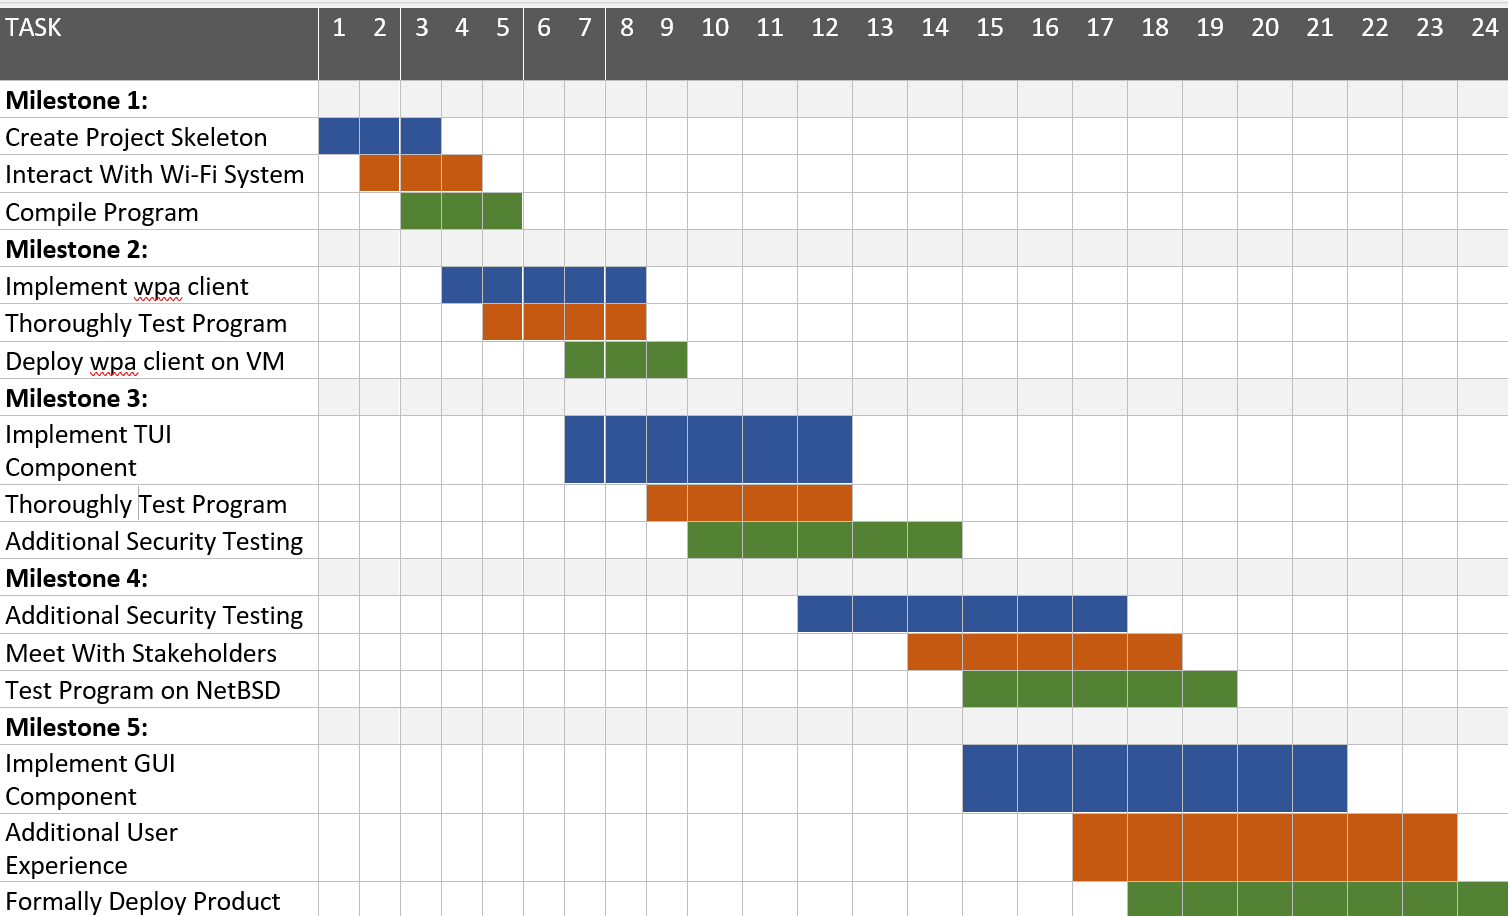
\includegraphics[scale=0.40]{ganttChart.png}
\end{figure}

\subsection{Key Milestones}
% Milestones are points in the development where you have implemented some
% number of major features.  For senior project, you generally have five
% milestones: one at the end of 491, three in 492, and one in 493.
% In this section, divide the Major Features between the milestones.  You should
% front-load the schedule as much as possible.  That is, leave 10% of the work
% for the last milestone.  

Milestone 1: Create skeleton of project. For this milestone, we should be able to compile something to test our project. With minor implementation. 
Milestone 2: Implement wpa client component of Wi-Fi. We can do security testing here, but to just make sure it works I think is okay. 
Milestone 3: Implement TUI component of Wi-Fi API. Since we should have the connection to Wi-Fi working in the previous milestone, we might be able 
to do more security testing here. 
Milestone 4: I think milestone 4 should be mostly security testing and meeting with stakeholders to get our project ready for deployment. We will have 
extra time during this milestone to test everything thoroughly. 
Milestone 5: If we have met all previous milestones and if time permits, we can work on the GUI component of our API. However, we will probably do more 
testing here to make sure everything works correctly. 

\subsection{Resource Assignments}
% Resources include budgets, consumables like paint, and computing equipment
% like servers and development systems.  Assign these resources, if any, to the
% tasks, listed above. 
%

Resources will include Western computers that can interact with NetBSD operating system so we can test our product. Additional resources will include 
additional computers to work on developing our project. Budgets and additional consumables I don’t think are needed here. 


\subsection{Individual Responsibilities}
% Who is responsible for which parts of the development effort.
%


\end{document}
